%
%  Erik Olsen
%
\documentclass[12pt,fullpage]{article}
\usepackage{fullpage}                                        % use all of the page for text 
\usepackage{psfrag}                                          % LaTeX graphics tool
\usepackage{pslatex}                                         % avoids the default cmr font
\usepackage{graphicx}                                        % graphics package 
\usepackage{epsfig}                                          % figures
\usepackage{epsfig} 
\usepackage{hyperref}
\usepackage{color}

\begin{document}

\noindent
{\bf Hypergeometric distribution}
(from \color{blue}\url{http://www.math.wm.edu/~leemis/chart/UDR/UDR.html}\color{black})

\noindent
The shorthand $X \sim$ hypergeometric$(n_1,\, n_2,\, n_3)$ is used to indicate
that the random variable~$X$ has the hypergeometric distribution for some
nonnegative integer parameters $n_1, n_2,$ and $n_3$,
where $n_1, n_2 \in \{ 0, 1, 2, ~\ldots,\, n_3\}$.
A hypergeometric random variable $X$ for parameters $n_1$, $n_2$, and $n_3$
has probability mass function 
$$
f(x) = \frac{{n_1 \choose x} {n_3 - n_1\choose n_2 - x}}{{n_3 \choose n_2}}.
$$
for $x = \max\{0,\, n_1 + n_2 - n_3\}, \ldots, \min\{n_1,\,n_2\}$.
The hypergeometric distribution is used for sampling without replacement from a
finite population of items. 
More specifically, a hypergeometric random variable $X$ is the number of
defective items in a sample of size $n_2$ items drawn at random and without
replacement from a lot of $n_3$ items which contains $n_1$ defective items.
Applications include acceptance sampling from quality control and animal
population size estimation using tagging with capture/recapture.
The probability mass function for $n_1 = 15$, $n_2 = 10$, and $n_3 = 50$
is illustrated below.

\begin{figure}[h!]
\psfrag{labx}{$x$}
\psfrag{labf}{$f(x)$}
\begin{center}
\includegraphics[width=4.2in]{HypergeometricPlot.ps}
\end{center}
\end{figure}

\noindent
The cumulative distribution function on the support of $X$ is
$$
F(x) = P(X \leq x) = \sum_{k = 0} ^ x \frac{{n_1 \choose k}
{n_3 - n_1 \choose n_2 - k}}{{n_3 \choose n_2}}\qquad \qquad
x=\max\{0, n_1 + n_2 - n_3\}, \ldots, \min\{n_1, \,n_2\}. 
$$
The moment generating function (from Wikipedia) of $X$ is 
$$
M_X(t) =
\frac{
{n_3 - n_1 \choose n_2}
}
{
{n_3 \choose n_2}
}
\, _ 2 F _ 1 \left( -n_2, \, -n_1, \, n_3 - n_1 - n_2 + 1, \, e ^ {\, t} \right),
$$
where $\, _ 2 F _ 1$ is the hypergeometric function defined by 
$$
\, _ 2 F _ 1 (a, \, b, \, c, \, z) =
1 + 
\frac{ab}{c} \cdot \frac{z}{1!} +
\frac{a(a+1)b(b+1)}{c(c+1)} \cdot \frac{z^2}{2!} +
\frac{a(a+1)(a+2)b(b+1)(b+2)}{c(c+1)(c+2)} \cdot \frac{z^3}{3!} + \cdots .
$$
The population mean, variance, and skewness of $X$ are
$$
E[X] = \frac{n_1 n_2}{n_3} \qquad \qquad
V[X]=\frac{n_2 n_1(n_3 - n_1)(n_3 - n_2)}{n_3 ^ 2(n_3 - 1)} \qquad \qquad
$$
$$
E\left[ \left( \frac{X - \mu}{\sigma} \right) ^ 3 \right] =
\frac{(n_3 - 2n_1)(n_3 - 1) ^ {1 / 2}(n_3 - 2n_2)}
{\left[n_2 n_1(n_3 - n_1)(n_3 - n_2)\right] ^ {1 / 2}(n_3 - 2)}. \qquad \qquad 
$$

\vspace{0.1in}

\newpage

\noindent
{\bf APPL verification:}
The APPL statements
%\begin{small}
%\begin{verbatim}
%assume(n_1 :: posint);
%assume(n_2 :: posint);
%assume(n_3 :: posint);
%additionally(n_3 > n_1);
%additionally(n_3 > n_2);
%X := [[x->(binomial(n_1, x) * binomial(n_3 - n_1, n_2 - x)) / binomial(n_3, n_2)], 
%       [max(0,n_1 + n_2 - n_3)..min(n_1, n_2)], ["Discrete", "PDF"]];
%\end{verbatim} \end{small}
%return the probability mass function using the parameterization used above.
%However, APPL has a built in function for the hypergeometric distribution as well.  The following statements
\begin{verbatim}
X := HypergeometricRV(n3, n1, n2);
Mean(X);
Variance(X);
Skewness(X);
\end{verbatim}
return complicated expressions for the population mean, variance, and skewness. 
\end{document}
